\documentclass[letterpaper]{article} % DO NOT CHANGE THIS
\usepackage[submission]{aaai2027}  % DO NOT CHANGE THIS
\usepackage[hyphens]{url}  % DO NOT CHANGE THIS
\usepackage{graphicx} % DO NOT CHANGE THIS
\urlstyle{rm} % DO NOT CHANGE THIS
\def\UrlFont{\rm}  % DO NOT CHANGE THIS
\usepackage{natbib}  % DO NOT CHANGE THIS AND DO NOT ADD ANY OPTIONS TO IT
\usepackage{caption} % DO NOT CHANGE THIS AND DO NOT ADD ANY OPTIONS TO IT
\frenchspacing  % DO NOT CHANGE THIS
\usepackage{booktabs}

\pdfinfo{
/TemplateVersion (2027.1)
}

\setcounter{secnumdepth}{1}

\title{Null-Attractor Attention: Thermodynamic Diagnostics for Jailbreak-Like Latent States}
\author{
    Anonymous Submission
}
\affiliations{
    %
}

\begin{document}

\maketitle

\begin{abstract}
% TODO: ~150-200 words. Draft last, after Sections 1-6 are stable.
% Must cover: (1) energy/Hopfield reading of attention + a risk-gated null attractor as a
% controlled perturbation; (2) basin-energy diagnostic scoring hidden states against
% safe/unsafe/benign anchors; (3) cross-model validation (unaligned GPT-2-family vs. aligned
% Qwen2.5-0.5B-Instruct) showing the diagnostics track trained refusal semantics, not an
% arbitrary property of attention; (4) a layer-scale confound found in the null-attractor
% mechanism itself via a risk=0 ablation, and its fix, which also measurably improved
% generation-time risk-selectivity; (5) an explicit negative-control result: detection is not
% yet solved safe generation control.
\end{abstract}

% \begin{links}
%     \link{Code}{ANONYMIZED}
% \end{links}

\section{Introduction}
% TODO (Task: Draft Intro/RelatedWork/Limitations/Conclusion/Abstract)

\section{Background and Related Work}
\label{sec:related}
% TODO. Source: docs/paper/related_work.md, docs/paper/related_work_basin_energy_synthesis.md.
% MUST re-verify arXiv:2605.02958 numbers against the primary source before citing (flagged
% during research as extracted via an automated PDF summary, not independently confirmed).

\section{Theory: Attention as a Two-Level Boltzmann System}
\label{sec:theory}

We first develop the theory that organizes the rest of the paper: a risk-gated null attractor
turns a self-attention head into an exactly solvable two-level Boltzmann system whose occupation
is the diagnostic observable. The theory unifies our two diagnostics, predicts a subtle baseline
confound before we observe it, and yields a testable prediction about where the response is most
sensitive. All three results below are verified numerically against our implementation to machine
precision (Sec.~\ref{sec:exp-depth}); throughout we distinguish an input's \emph{risk}
$R(X)\in[0,1]$ from the model's \emph{response} to a perturbation gated by that risk, and our
claims concern the response.

\subsection{The Null Attractor as an Exact Two-Level System}
\label{sec:theory-order}
For queries $Q$, keys $K$, values $V$ and scaling $s=1/\sqrt{d_k}$, standard attention assigns
$p_{ij}\propto\exp(\beta\,s\,q_i^\top k_j)$, the Boltzmann reading $E_{ij}=-s\,q_i^\top k_j$,
$p_{ij}\propto\exp(-\beta E_{ij})$
\citep{ramsauer2020hopfield,hoover2023energytransformer,santos2024hopfieldfenchelyoung}. We append
one synthetic \emph{null} slot $(k_{\text{null}},v_{\text{null}})$ and gate its energy on risk. For
query $i$ the extended logits are
%
\begin{equation}
z_{ij} = \beta(R)\bigl(s\,q_i^\top k_j - \lambda R\,\Phi_{ij} + b_j\bigr),
\label{eq:logits}
\end{equation}
%
with a null bias $b_{\text{null}}=\eta\,g_R$ applied only to the null slot ($b_j=0$ otherwise),
gate $g_R=\sigma(\kappa(R-R_c))$, critical risk $R_c$, and $\beta(R)$ interpolating
$\beta_{\text{base}}\!\to\!\beta_{\text{collapse}}$ under the same gate. The order parameter is the
null mass $m_{\text{null}}=\frac1n\sum_i p_{i,\text{null}}$.

Summing the softmax over the $n$ real keys and the one null slot collapses to a closed form. Let
$z^{\text{null}}_i=s\,q_i^\top k_{\text{null}}$ be the bare null logit and let
$F_i=\frac1\beta\log\sum_{j}\exp(\beta\,s\,q_i^\top k_j)$ be the free energy of the real keys.
Then the per-query null mass is exactly
%
\begin{equation}
m_{\text{null},i} = \sigma\!\bigl(\beta(R)\,[\,\Delta_i + \eta\,g_R + \lambda R\,]\bigr),
\qquad \Delta_i = z^{\text{null}}_i - F_i,
\label{eq:orderparam}
\end{equation}
%
where $\sigma$ is the logistic function. The head is thus a two-level system: the null state
competes against the aggregated real-key state, and $m_{\text{null}}$ is its Fermi-like occupation.
The bare gap $\Delta_i$ sets the operating point; the risk field enters through $\eta g_R$ (bias)
and $\lambda R$ (penalty), and $\beta(R)$ sharpens the response. We verify Eq.~\eqref{eq:orderparam}
against the implementation to a maximum error of $3.3\times10^{-16}$ over random configurations.

\subsection{Susceptibility and a Shifted Critical Point}
\label{sec:theory-chi}
The diagnostic signal is the response's sensitivity to risk. In the constant-$\beta$,
$\lambda{=}0$ regime, differentiating Eq.~\eqref{eq:orderparam} gives the susceptibility
%
\begin{equation}
\chi(R)=\frac{\mathrm{d}\,m_{\text{null}}}{\mathrm{d}R}
= \beta\eta\kappa\; m_{\text{null}}(1-m_{\text{null}})\; g_R(1-g_R),
\label{eq:chi}
\end{equation}
%
a product of two bump factors whose height scales with $\beta\eta\kappa$. Its peak---the critical
point of the observable---does not sit at the nominal gate midpoint $R_c$ but is shifted by the
bare gap: $m(1-m)$ is maximal where $\eta g_R=-\Delta$, i.e.\ at $R<R_c$ when the null state starts
disfavored ($\Delta<0$). This is a concrete, falsifiable prediction; Sec.~\ref{sec:exp-depth}
confirms both the closed form (to $1.7\times10^{-4}$ vs.\ finite differences) and the sub-$R_c$
peak.

\subsection{The Baseline Confound Is a Theorem}
\label{sec:theory-confound}
Eq.~\eqref{eq:orderparam} exposes a trap that no amount of tuning would reveal. The null slot needs
a bare logit $z^{\text{null}}_i$. The natural first choice---a constant (e.g.\ $k_{\text{null}}=0$,
so $z^{\text{null}}_i=0$)---makes the operating point $\Delta_i=-F_i$ track the real-key free
energy, which varies across layers for reasons unrelated to risk. Under a uniform additive shift of
the real logits by $c$ (a layer sitting at a different offset), $F_i\mapsto F_i+c$, so even at
$R{=}0$ the baseline $m_{\text{null}}$ moves. Raw null mass then conflates risk-driven attraction
with a layer-specific baseline, and any layer selected by raw magnitude is suspect.

The fix follows directly from Eq.~\eqref{eq:orderparam}: set the null logit to the mean real logit,
$z^{\text{null}}_i=\frac1n\sum_j s\,q_i^\top k_j$. Both this mean and $F_i$ shift by the same $c$
under an additive offset, so $\Delta_i$---and hence $m_{\text{null}}$---is \emph{exactly invariant}
(we confirm machine-zero spread numerically). We therefore report a mandatory \emph{risk=0
ablation}: rerun with the gate forced shut and subtract the residual baseline separation, reporting
the risk-attributable $\mathrm{sep}(m_{\text{null}})_{\text{real}}-\mathrm{sep}(m_{\text{null}})_{R=0}$.
That a baseline control is necessary is not incidental to our system---it is what
Eq.~\eqref{eq:orderparam} predicts for any additively-referenced attractor observable.

\subsection{Unification: Diagnostics as Occupation of an Augmented State Space}
\label{sec:theory-unify}
The same structure governs our semantic diagnostic. Given a pooled hidden state $h(X)$ and basin
centroids $c_b$ for $b\in\{\text{safe},\text{unsafe},\text{benign}\}$, define basin energies
$E_b(X)=-\cos(h(X),c_b)$ and the Boltzmann occupancy $P(b\mid X)\propto\exp(-E_b/T)$
\citep{ctm2023cosine}, with free energy $F=-T\log\sum_b\exp(-E_b/T)$ and basin entropy
$S=-\sum_b P(b\mid X)\log P(b\mid X)$. The null attractor and the basin-energy diagnostic are then
the same object---Boltzmann occupation of an augmented state space (an appended slot; a set of
semantic basins)---with risk acting as a field that tilts the occupation and the observable being
the target basin's order parameter. The safe-vs-unsafe competition is the margin $\Delta
E=E_{\text{unsafe}}-E_{\text{safe}}$, with selectivity $\mathrm{sep}(\Delta E)=
\mathbb{E}[\Delta E\mid\text{jailbreak}]-\mathbb{E}[\Delta E\mid\text{benign}]$.

Because a single mean-difference anchor assumes refusal is one-dimensional---false, as refusal is
mediated by a multi-dimensional cone \citep{wollschlager2025geometry,moreThanSingleDirection2026}---we
additionally estimate a refusal/unsafe \emph{subspace} from several anchor pairs via SVD, orient its
primary axis to the mean-difference direction (SVD signs are arbitrary), and report both margins.
Their agreement is itself diagnostic: if one direction sufficed, the two would correlate positively.

\paragraph{Crossover vs.\ transition.} A single head is a smooth crossover, not a true phase
transition: Eq.~\eqref{eq:orderparam} is analytic for finite $\beta$. A genuine transition would
require collective coupling---many query positions, heads, and layers sharing $R(X)$, which itself
depends on the hidden state that the attractor reshapes. Our toy system approaches this mean-field
limit and shows a sharp jump; real models show only partial transfer
(Sec.~\ref{sec:exp-prior}). We are careful to claim a crossover with phase-transition-\emph{like}
sharpening in $\beta\eta\kappa$, not a thermodynamic singularity.

\section{Method}
\label{sec:method}
We operationalize the theory as two diagnostics over a fixed set of prompt suites. The null
attractor is implemented as an in-layer patch to the eager-attention path of Hugging Face causal
LMs; the patch reconstructs the extended logits of Eq.~\eqref{eq:logits}, expands grouped-query
key/value heads so the same code runs on multi-head (GPT-2) and grouped-query (Qwen2) attention,
and logs $m_{\text{null}}$, entropy $H=-\sum_j p_{ij}\log p_{ij}$, and a spectral-gap concentration
proxy per layer and head. The null logit uses the mean-logit reference of
Sec.~\ref{sec:theory-confound} by default, and every depth sweep is paired with its risk=0 control.
The basin-energy diagnostic is post-hoc: we mean-pool a chosen layer's hidden states, score them
against anchor centroids and the oriented refusal/unsafe subspace, and report the margins and their
agreement. Both diagnostics are risk-agnostic in the sense that basin energy needs no $R(X)$ at all,
and the null attractor's response is measured relative to its own risk=0 baseline; we treat the
prompt-level $R(X)$ as a transparent scaffold rather than a contribution.

\section{Experiments}
\label{sec:experiments}

\paragraph{Setup.} We evaluate two models with deliberately different training: \texttt{distilgpt2}
(6 layers, multi-head attention, no RLHF or safety tuning) and \texttt{Qwen2.5-0.5B-Instruct}
(24 layers, grouped-query attention, RLHF/safety-tuned) \citep{qwen2025technicalreport}. Prompts
are drawn from eight fixed suites---benign, benign-complex, direct/obfuscated/long-context/
many-shot jailbreak, paraphrased-adversarial, and safety-research---labeled jailbreak or benign;
all harmful examples are non-operational. Basin anchors are three short natural-language prompts
(a refusal, a compliant-unsafe, and a benign completion); the refusal/unsafe subspace is estimated
from four additional refusal-minus-unsafe pairs. Unless noted, risk uses a transparent surface
heuristic, which we treat as a scaffold (Sec.~\ref{sec:limitations}); the diagnostics themselves
are risk-agnostic.

\subsection{Prior Diagnostic Evidence}
\label{sec:exp-prior}
The mechanism's phase behavior is established in a toy energy system and in post-hoc real
hidden-state diagnostics (Table~\ref{tab:prior}). The toy system shows the intended sharp
order-parameter jump ($m_{\text{null}}$ rising from $0.075$ to $0.999$ across $R_c$); a normalized
\texttt{distilgpt2} diagnostic shows a steep but imperfect transfer, and a \texttt{tiny-gpt2}
diagnostic shows none, exposing that risk must be a latent-trajectory functional rather than a
surface heuristic before magnitudes are comparable across settings. These are mechanism tests, not
in-layer interventions, and we report them only as scaffolding for the cross-model results below.

\begin{table}[t]
\centering
\begin{tabular}{lccc}
\toprule
setting & low-risk $m_{\text{null}}$ & high-risk $m_{\text{null}}$ & jump \\
\midrule
toy                       & 0.075 & 0.999 & 0.924 \\
tiny-gpt2 diag.\          & 0.035 & 0.033 & $-0.002$ \\
distilgpt2 diag.\ (norm.) & 0.558 & 0.999 & 0.441 \\
\bottomrule
\end{tabular}
\caption{Prior phase-transition evidence (mechanism tests, not interventions). The toy jump is
sharp; real-model transfer is partial and confounded by excess low-risk mass---motivating the
baseline control in Sec.~\ref{sec:exp-depth}.}
\label{tab:prior}
\end{table}

\subsection{Cross-Model Basin-Energy Validation}
\label{sec:exp-basin}
We sweep the basin-energy diagnostic across layers of both models
(Fig.~\ref{fig:basin}). The raw separation magnitude $\mathrm{sep}(\Delta E)$ is small and
comparable across models ($0.004$--$0.018$ on \texttt{distilgpt2}, up to $0.013$ on Qwen), so
magnitude alone does not distinguish them. The distinguishing signal is the agreement between the
single-anchor and subspace primary-axis margins. On \texttt{distilgpt2} the two disagree at nearly
every layer (correlation $-0.41$ to $-0.87$, one near-zero), consistent with no coherent refusal
axis to recover. On Qwen the two agree strongly and depth-dependently (correlation $0.80$ to
$0.97$ across layers 6--21), and the separation grows monotonically to a peak at layer 21 before
collapsing in the final two layers. The collapse coincides with a known attention-sink /
compression-valley regime \citep{attentionSinkEmerges2025,compressionValleys2025} and is a
property of the final layers, not of the diagnostic. That a diagnostic built from generic
cosine-to-anchor energies produces a coherent, depth-structured signal on an aligned model and
noise on an unaligned one is our central evidence that it tracks trained refusal semantics rather
than an arbitrary property of attention.

\begin{figure}[t]
\centering
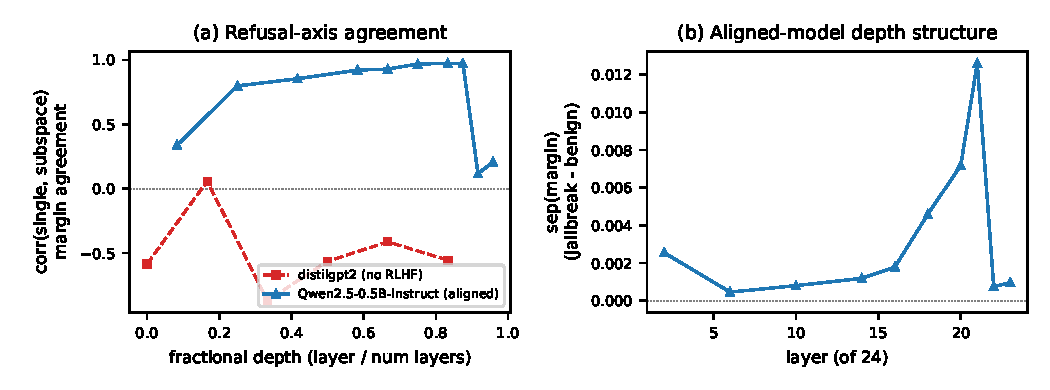
\includegraphics[width=0.98\columnwidth]{figures/basin_energy_depth}
\caption{Cross-model basin energy. (a) Agreement between the single-anchor and subspace
primary-axis margins vs.\ fractional depth: the aligned model (Qwen) agrees strongly then
collapses at the end; the unaligned model (distilgpt2) mostly disagrees. (b) On Qwen, basin
separation rises through the mid-to-late layers and collapses at layers 22--23.}
\label{fig:basin}
\end{figure}

\subsection{Null-Attractor Depth and the Risk=0 Ablation}
\label{sec:exp-depth}

\paragraph{Theory verification.} Before the model sweeps, we confirm the theory of
Sec.~\ref{sec:theory} against the implementation. The two-level closed form
(Eq.~\eqref{eq:orderparam}) matches measured per-query null mass to a maximum error of
$3.3\times10^{-16}$ over $200$ random configurations; the susceptibility formula
(Eq.~\eqref{eq:chi}) matches finite differences to $1.7\times10^{-4}$ and its peak sits at
$R=0.446$ below the gate midpoint $R_c=0.5$, as predicted; and the mean-logit reference makes
$m_{\text{null}}$ exactly invariant (machine-zero spread) to additive logit shifts that move the
constant-reference baseline by up to $0.15$. These checks are permanent regression tests.

We next sweep the null-attractor diagnostic across Qwen's layers, with the automatic risk=0
control (Sec.~\ref{sec:theory-confound}). Under the original constant null logit, the baseline term is
large and layer-dependent: at layer 21---the layer the uncontrolled metric selected as
``best''---$77\%$ of the raw jailbreak $m_{\text{null}}$ ($0.72$) is present even with the risk
gate forced shut, and the baseline fraction ranges from $7\%$ to $83\%$ across layers. Reading raw
$m_{\text{null}}$ magnitude or selecting a layer from it is therefore unsafe.

The \texttt{mean\_logit} fix removes the confound (Fig.~\ref{fig:fix}). The baseline fraction
becomes a stable $6.7\%$--$8.3\%$ at every layer, and the risk-attributable separation is
substantial and roughly flat across the usable depth range ($0.17$--$0.26$), peaking at layer 10
($0.257$) rather than the layer 21 the confounded metric preferred. Entropy separation is negative
at all ten tested layers (jailbreak attention is consistently more concentrated than benign),
a depth-robust signal that does not depend on the null-slot design. We stress that the pre- and
post-fix curves disagree on both the peak layer and the presence of a final-layer collapse; an
earlier cross-diagnostic ``agreement'' between $m_{\text{null}}$ and basin energy at layers 22--23
did not survive the fix and we do not claim it.

\begin{figure}[t]
\centering
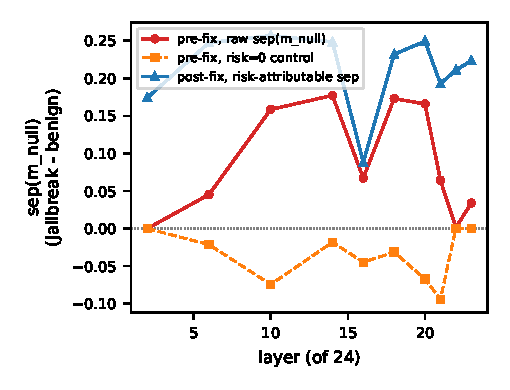
\includegraphics[width=0.82\columnwidth]{figures/null_attractor_depth_fix}
\caption{Null-attractor depth diagnostic on Qwen. The pre-fix raw separation (red) is inflated by
a layer-dependent baseline (orange, risk=0 control). The post-fix risk-attributable separation
(blue) is flat across depth and peaks at layer 10.}
\label{fig:fix}
\end{figure}

\subsection{Generation Intervention: A Negative Control}
\label{sec:exp-gen}
Finally we run the intervention at generation time on Qwen, whose untouched baseline already
refuses jailbreak prompts and answers benign prompts fluently---the first setting in this line of
work where the baseline is not itself broken, making this a sharp test. At the confounded layer 21,
every null-value mode (empty, refusal-semantic, redirection-semantic) drove benign $m_{\text{null}}$
to $0.6$--$0.7$, nearly as high as jailbreak, and degraded all continuations into token loops. At
the corrected layer 10, risk-selectivity improves sharply: benign and safety-research
$m_{\text{null}}$ fall to $\approx 0.01$ while jailbreak/obfuscated reach $0.40$--$0.62$, and the
semantic modes produce a correct refusal token (``No.'') on jailbreak prompts where the empty sink
drifts toward an affirmative (``Yes''). A repetition-controlled rerun confirms the refusal signal
is genuine content rather than a loop artifact, but also reveals that benign coherence still breaks
at $\approx 1\%$ null mass---run-together, malformed text rather than merely repetitive output.
Fixing the mechanism thus measurably improved risk-selectivity and the semantics of the induced
signal, but did not yield safe generation: detection is not solved control.

\section{Limitations}
\label{sec:limitations}
% TODO. Source: docs/paper/limitations.md, updated with: benign coherence break confirmed
% under repetition control; single aligned model tested; small suite sizes; refusal known to
% be multi-dimensional (cones) and not fully captured by a mean-difference anchor.

\section{Conclusion}
% TODO. Source: docs/paper/outline.md Sec 6.

\section*{Ethical Statement}
% TODO: short paragraph. All harmful-prompt examples used in this work are non-operational
% and drawn from a fixed benchmark suite (thermosafety/prompts/*.jsonl); no operational
% jailbreak payloads are disclosed.

% References and End of Paper
% These lines must be placed at the end of your paper
\bibliography{references}

% \input{ReproducibilityChecklist.tex}

\end{document}
